\documentclass[conference]{IEEEtran}
\IEEEoverridecommandlockouts
% The preceding line is only needed to identify funding in the first footnote. If that is unneeded, please comment it out.
\usepackage{cite}
\usepackage{amsmath,amssymb,amsfonts}
\usepackage{algorithmic}
\usepackage{graphicx}
\usepackage{textcomp}
\usepackage{xcolor}
\usepackage{url} 
\usepackage{listings}
\usepackage{blindtext}
\usepackage[most]{tcolorbox}
\usepackage{subcaption}
\usepackage{float}
\usepackage{hyperref}

\makeatletter
\NewDocumentCommand{\mynote}{+O{}+m}{%
  \begingroup
  \tcbset{%
    noteshift/.store in=\mynote@shift,
    noteshift=1.5cm
  }
  \begin{tcolorbox}[nobeforeafter,
    enhanced,
    sharp corners,
    toprule=1pt,
    bottomrule=1pt,
    leftrule=0pt,
    rightrule=0pt,
    colback=yellow!20,
    #1,
    left skip=\mynote@shift,
    right skip=\mynote@shift,
    overlay={\node[right] (mynotenode) at ([xshift=-\mynote@shift]frame.west) {\textbf{Note:}} ;},
    ]
    #2
  \end{tcolorbox}
  \endgroup
  }
\makeatother

\def\BibTeX{{\rm B\kern-.05em{\sc i\kern-.025em b}\kern-.08em
    T\kern-.1667em\lower.7ex\hbox{E}\kern-.125emX}}

\usepackage{xcolor}

\definecolor{codegreen}{rgb}{0,0.6,0}
\definecolor{codegray}{rgb}{0.5,0.5,0.5}
\definecolor{codepurple}{rgb}{0.58,0,0.82}
\definecolor{backcolour}{rgb}{0.95,0.95,0.92}

\lstdefinestyle{mystyle}{
    backgroundcolor=\color{backcolour},   
    commentstyle=\color{codegreen},
    keywordstyle=\color{magenta},
    numberstyle=\tiny\color{codegray},
    stringstyle=\color{codepurple},
    basicstyle=\ttfamily\footnotesize,
    breakatwhitespace=false,         
    breaklines=true,                 
    captionpos=b,                    
    keepspaces=true,                 
    numbers=left,                    
    numbersep=5pt,                  
    showspaces=false,                
    showstringspaces=false,
    showtabs=false,                  
    tabsize=2
}

\lstset{style=mystyle}

    
\begin{document}

\title{CS598 CCC Final\\
}

\author{
\IEEEauthorblockN{Cameron Greenwalt}
\IEEEauthorblockA{
\textit{UIUC}\\
Champaign, IL, USA \\
cg50@illinois.edu}
\and
\IEEEauthorblockN{Ming Meng}
\IEEEauthorblockA{
\textit{UIUC}\\
Champaign, IL, USA \\
mingm4@illinois.edu}
\and
\IEEEauthorblockN{Yang Peng}
\IEEEauthorblockA{
\textit{UIUC}\\
Champaign, IL, USA \\
yangp3@illinois.edu}
}
\maketitle


\begin{abstract}
Artificial Intelligence for IT Operations (AIOps) is re-defining incident resolution in cloud computing. This project highlights the significance of employing AI methods in log analysis and produce log summaries. It aims to expedite the diagnosis of cloud application issues through human readable generated log summaries through Large Language Models. AIOps aims to minimize cloud system downtime and therefore improves organization efficiencies which leads to improvements in customer satisfaction.
\end{abstract}

\section{Introduction} \label{sec:introduction}

Artificial Intelligence for IT Operations (AIOps) is the field in which AI methods are used to solve common IT problems. Use of AIOps in organizations of all sizes is appealing because AIOps has the potential to accelerate the resolution process of IT problems. The cloud computing field is prone to incidents that require IT expertise and resources to resolve, as applications deployed onto cloud systems are often complex. In the event that an incident occurs in an organization's cloud application, the site reliability engineers (SREs) tasked with resolving the incident are likely to encounter difficulty in diagnosing a root cause for the cloud application's faulty state. \cite{chen2020aiops} \cite{mani2023enhancing}

In the process of diagnosing a cloud incident's root cause, the SREs will analyze logs from applications and services involved in the incident. The objective in analyzing cloud logs is to assess application state, determine the inputs that led to that state, and trace what other services could have been affected by that state. The task of analyzing logs is arduous and slow because logs often are verbose, difficult to parse, numerous, and not human-reader friendly. If AI can be used to effectively accelerate this process of log analysis, then SREs can diagnose incidents more efficiently and businesses can expect to reduce costs and increase profits. \cite{10212414} \cite{gupta2023learning} Cloud system downtime creates dissatisfied customers and wasteful overhead as compute resources are provisioned but not used to generate revenue. \cite{li2022an} Reducing the amount of time required for SREs to diagnose cloud incidents will lead to shorter and less frequent cloud application downtime, which in turn leads to greater revenue generation.

We have made our code and implementation available on \href{https://github.com/mingmcs/cs598ccc}{GitHub}. \footnote{https://github.com/mingmcs/cs598ccc}

\subsection{Background and Motivation}

The application of AI methods to solve IT problems is often expensive. \cite{LEE2023110689} \cite{network-log-anomaly-detection} AI solutions often necessitate teams of machine learning experts that know how to train, deploy, and maintain AI models. \cite{aiops-challenges} AI model training can be prohibitively expensive--even in cases where models are fine-tuned using domain-specific data rather than trained from scratch. Any AI model that can be deployed and provide acceptable use-case performance without a prerequisite training step on domain-specific data is preferable to a model that does require such training. Therefore, we would like to minimize the amount of training and fine-tuning required to use an AI model to analyze logs. We plan to do this by utilizing existing pre-trained large language models (LLMs).

\subsection{Our Solution}

In this research, we aim to accelerate the rate at which SREs can analyze logs by using natural language processing (NLP) LLMs to summarize cloud application logs, thus providing SREs with shorter and more easily understood and parsed representations of logs, which representations will retain the critical information contained within the original logs. \cite{medium-text-summarization} Specifically, we will use the ChatGPT family of LLMs to generate the log summaries. We plan to boost the the quality of generated log summaries by providing ChatGPT with additional contextual understanding of log semantics by embedding domain-specific text with the ADA embedding model and using the resultant embedding vectors as additional input to ChatGPT. We hypothesize that doing so will improve model performance in a particular domain (e.g., logs belonging to one type of application such as Apache Zookeeper) without requiring prior training or fine-tuning steps. In other words, the ChatGPT model parameters will remain unchanged.

Our solution will be a cloud-based, chat-oriented application hosted on Microsoft's Azure cloud hosting platform. The application will use the Azure OpenAI Service API to perform text embedding and ChatGPT inference steps.

\subsection{Evaluation}


We evaluate the quality of the generated log summaries by summarizing logs from Apache Zookeeper \cite{zookeeper} calculating several NLP text generation evaluation metrics on the generated summaries. In previous milestones, we had said we would logs from the Proxifier \cite{proxifier} application, but we have since pivoted to using Zookeeper logs because they are more diverse and information-rich than Proxifier logs. The metrics for evalutation that we compute include ROUGE \cite{lin2004rouge}, BERTScore \cite{bert-score}, BLEURT \cite{sellam2020bleurt}, BLEU \cite{10.3115/1073083.1073135}, NUBIA \cite{kane2020nubia}, and METEOR \cite{banerjee-lavie-2005-meteor}. Additionally, we perform log summarization using other baseline methods and assess the effectiveness of our proposed solution to that of the baseline methods by comparing the values of the previously listed metrics for both our solution and the baseline methods.

\subsection{Contribution}

The summary of our major contributions is as follows:

\begin{itemize}
    \item We implement a novel method for summarizing cloud application logs using the ChatGPT family of generative models.
    \item We provide ChatGPT with deeper understanding of cloud application logs by embedding domain/application-specific text using the ADA embedding model and using the resulting vector embeddings to provide additional prompt input to ChatGPT.
    \item Our solution is a chat-based approach to generating log summaries. Chat-based approaches are accessible for experts and non-experts alike and can be adapted to be more scalable and automated.
\end{itemize}

\section{Prior work- Literature Survey}

Many prior research works have addressed the topic of log summarization. LogSummary \cite{10017337} is perhaps the work in closest relation to what we would like to accomplish in our research. LogSummary is an automatic and unsupervised log summarization framework that achieves an impressive ROUGE F1 score. The authors, upon finding that no"gold standard" labelled dataset of logs and their associated summaries exists, created their own dataset of logs and log summaries. They used this dataset to assess the quality of their models. We will use their open-source dataset in our work to assess the quality of our methods.

At the core of LogSummary is the LogIE algorithm, which "performs open information extraction on logs, extracting triples relating entities and arguments through relation or predicate." \cite{10017337} LogSummary does \textit{not} use generative LLMs such as ChatGPT, BERT, or derivatives. Rather, it uses a rule-based approach to extract information from logs. We plan to use LLMs to accomplish a similar objective while not being constrained to this research work's entities-events-relation triple output summary format or including complicated logic.

Some authors acknowledge that the ChatGPT model is more accurate than many other open source models that are presently available for summary generation. Additionally, ChatGPT often generates acceptable results without requiring a fine-tuning step prior to running inference. Presently, ChatGPT is the gold standard for most generative NLP tasks.\cite{bendimerad2023onpremise}

LogRule \cite{logrule} is a Root Cause Analysis (RCA) algorithm that offers a time-efficient, accurate, and interpretable solution for RCA in complex datasets--especially where the current state-of-the-art algorithm struggles with execution times. LogRule aims to provide an explanation for specific events of interest, but it depends on structured rather than unstructured logs, which means that doing log preprocessing or overhauling a system's logs to all be structured are prerequisites to using the system.

CloudRCA is "a root cause analysis framework for Alibaba Cloud's big data cloud computing platforms, utilizing heterogeneous multi-source data, state-of-the-art anomaly detection, and log analysis techniques to extract features, which are then employed in a Knowledge-informed Hierarchical Bayesian Network (KHBN) model." \cite{10.1145/3459637.3481903} CloudRCA is a thorough, useful system that is in-use in Alibaba's cloud systems. The authors claim that CloudRCA has provided a 20\% time savings for site reliability engineers (SREs). The cost for an organization to implement CloudRCA or a similar system in their own cloud platforms may exceed its relative benefit as it is quite niche and may not be generally applicable to dissimilar use cases. We envision that our work will have more general applicability and lower implementation cost for various organizations at the expense of narrower scope of operations, focusing on only the log summarization step of the incident analysis pipeline.

In \cite{10172904}, researchers showed that LLMs are effective in both identifying an incident's root cause and suggesting mitigation steps for the incident. This gives us confidence to proceed in our ChatGPT-based log summarization research.

BERT is a popular LLM alternative to ChatGPT that is used in cloud log-related tasks. BERT can be successful in performing specific tasks such as detection and classification but suffers from a lack of generalizability to different problem scopes. In addition, tasks using BERT and its derivatives often require training and fine-tuning steps. We have discussed previously that we do not want to perform any pre-training steps to obtain a useful model.

The performance of the anomaly log detection task using fine-tuned BERT-based models has proven to be very successful in recent research. For example, in one study, researchers were able to achieve an F1 score above 0.9 in detecting anomalies in a sample HDFS log dataset. This success can be attributed to the fact that HDFS log data is more structured than unstructured. In fact, the authors found that pre-training BERT with more natural language data had a negative impact on anomaly detection. \cite{LEE2023110689} From these researchers' experience, we hypothesize that ChatGPT may be better suited for logs with more natural language semantics.

In another study, the authors used the RoBERTa, a BERT derivative. The authors fine-tuned their model on both external and internal datasets, often borrowing popular new websites and articles. \cite{saha2022mining}

Another team of researchers used BERT-based models to build an intelligent-based system for IT Incident Operations. However, the metric scores they achieved with the base BERT models were quite low and often required additional classifiers such as LSTMs to increase accuracy. The complexity of this system might lead to over-fitting issues. \cite{10189040} We would like our system to involve as little complexity as possible.

In assessing the viability of using GPT models for log- and cloud-related tasks, researchers at Microsoft studied over 40,000 incidents from 1000+ cloud services with six semantic and lexical metrics.\cite{10172904}  The following are the key insights from their work:
\begin{itemize}
    \item Fine-tuning significantly improves the effectiveness of LLMs for incident data.
    \item GPT-3 and GPT-3.5 models significantly outperform encoder-decoder models in various experiments.
    \item Metrics such as BLEU-4 are useful for measuring relative performance of models in different settings. However, manual inspection and validation with experts is required to assess actual performance.
\end{itemize}

Since we would like to preserver the natural language characteristics of the input/output data and minimize the complexity of our application, we will use ChatGPT instead of BERT or similar NLP models to perform the log summarization task. 

The performance of LLMs in log related tasks can be improved by providing the models with more contextual data to use during inference. For example, log data can be used in conjunction with previous incident data to benefit incident management and resolution tasks.

Log data from user input alone may not offer enough insights to produce high-quality generated responses from ChatGPT. Technical documentations, knowledge articles, and/or past incident investigations data can be used to provide contextual information to AIOps tasks, thereby improving task performance. Some examples of these kinds of data include a company's internal root cause knowledge source database, technical documentation of the application or related systems, troubleshooting guides, and software release notes. These data are often unstructured but are beneficial for the generation of analysis and summaries. \cite{saha2022mining}



\section{Methods}

\subsection{Overview}

Our system will be known as "A general AIOps framework on log data using LLM-generated results". The system involves a user passing sample log data to our prompt generator application, which will vectorize the provided logs and store them in a vector store. Then, users will submit a natural language query to the chatbot such as "Summarize this log for me: [log]". The chatbot then generates a prompt by utilizing the existing query embeddings from the vector store. We then validate the generated result by computing metrics mentioned in Section \ref{sec:introduction}.

\begin{figure*}[ht]
    \centering
    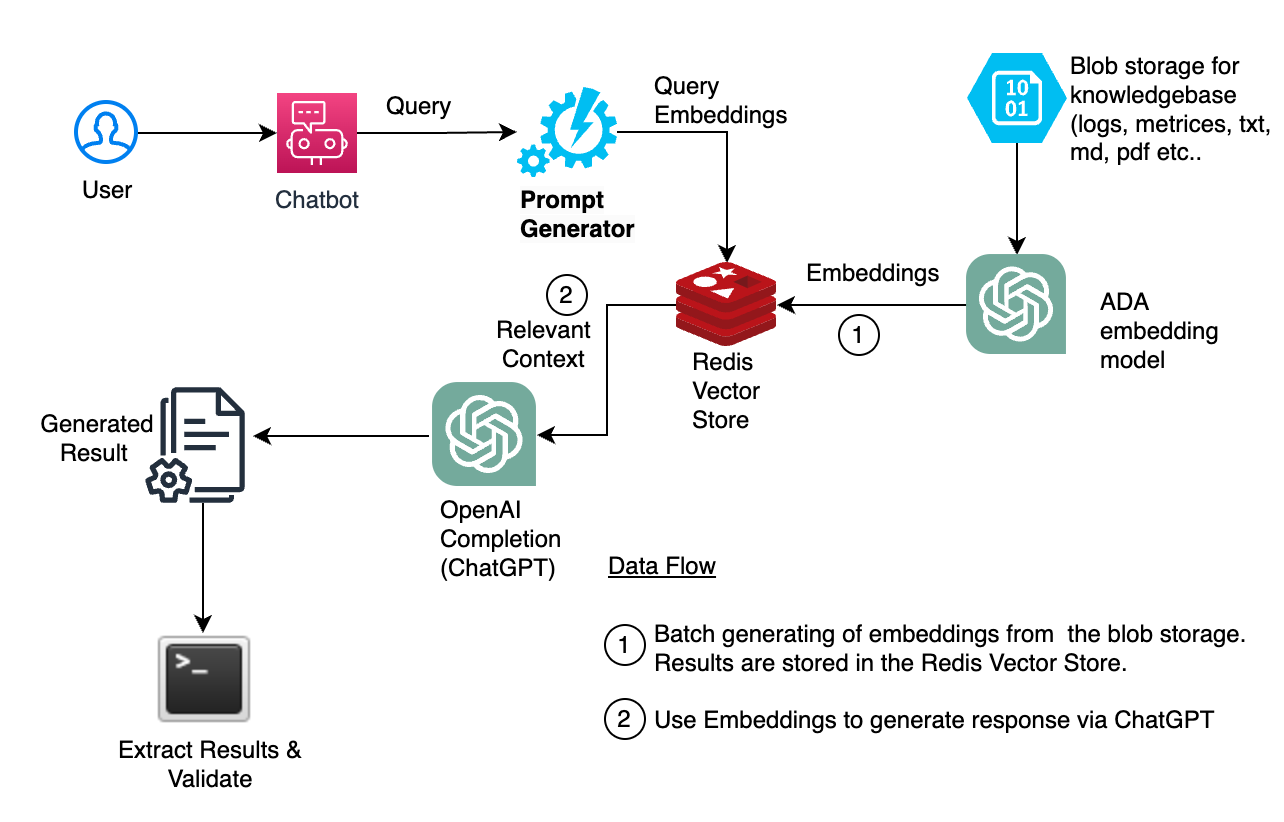
\includegraphics[width=0.8\textwidth]{arch.png}
    \caption{Our proposed AIOps framework using LLM-generated results}
    \label{fig:arch}
\end{figure*}

Figure \ref{fig:arch} above shows the proposed implementation of the system. The chatbot can be either UI or API based. In the following subsections, we detail each step of the system more concretely.


\subsection{Log Data}

We use a set of 100 logs from the Apache Zookeeper \cite{zookeeper} application made available on the LogHub GitHub repository \cite{zhu2023loghub} and the corresponding triples summaries generated in the LogSummary \cite{10017337} work (known henceforth as reference summaries). We perform a randomized 75/25 train-test split of the logs and their corresponding reference summaries. The training logs/reference summaries are used to populate the vector store (see Section \ref{subsec:vectorstore}) and the test logs/reference summaries are used in prompts and inference (see Section \ref{subsec:inference}. We separate the logs used to populate the vector store from those used in inference to avoid biasing the inference by performing a similarity search for a log that already exists in the vector store, thereby giving ChatGPT the reference summary in the prompt where we ask ChatGPT to summarize the log.

Listing \ref{lst:zookeeper-example} shows an example of one Zookeeper log and listing \ref{lst:zookeeper-summary} shows the reference summary for that log (generated by LogSummary).

\begin{figure*}[ht]
\begin{lstlisting}[numbers=none, caption=Zookeeper Log Example, label={lst:zookeeper-example}]
INFO Accepted socket connection from /10.10.34.11 : 49242
WARN Connection request from old client /10.10.34.11 : 49242 ; will be dropped if server is in r-o mode
INFO Client attempting to establish new session at /10.10.34.11 : 49242
INFO Accepted socket connection from /10.10.34.11 : 49244
WARN Connection request from old client /10.10.34.11 : 49244 ; will be dropped if server is in r-o mode
INFO Client attempting to establish new session at /10.10.34.11 : 49244
INFO Established session 0x14ed93111f20037 with negotiated timeout 10000 for client /10.10.34.11 : 49242
INFO Established session 0x14ed93111f20038 with negotiated timeout 10000 for client /10.10.34.11 : 49244
INFO Accepted socket connection from /10.10.34.13 : 37196
WARN Connection request from old client /10.10.34.13 : 37196 ; will be dropped if server is in r-o mode
INFO Client attempting to establish new session at /10.10.34.13 : 37196
INFO Established session 0x14ed93111f20039 with negotiated timeout 10000 for client /10.10.34.13 : 37196
INFO Accepted socket connection from /10.10.34.12 : 45605
WARN Connection request from old client /10.10.34.12 : 45605 ; will be dropped if server is in r-o mode
INFO Client attempting to establish new session at /10.10.34.12 : 45605
INFO Established session 0x14ed93111f2003a with negotiated timeout 10000 for client /10.10.34.12 : 45605
INFO Accepted socket connection from /10.10.34.13 : 37199
WARN Connection request from old client /10.10.34.13 : 37199 ; will be dropped if server is in r-o mode
INFO Client attempting to establish new session at /10.10.34.13 : 37199
INFO Established session 0x14ed93111f2003b with negotiated timeout 10000 for client /10.10.34.13 : 37199
\end{lstlisting}
\end{figure*}

\begin{figure}[ht]
\begin{lstlisting}[numbers=none, caption=LogSummary Zookeeper Summary, label={lst:zookeeper-summary}]
 Accepted socket connection;Connection request will be dropped; Client attempting to establish new session; Established session timeout;
\end{lstlisting}
\end{figure} 


\subsection{Knowledgebase - Domain Context Vector Embedding} \label{subsec:vectorstore}

We vectorize individual logs from the corpus of 75 Zookeeper logs using the \lstinline{text-embedding-ada-002} ADA embedding model in the Azure OpenAI Service API. We then populate a Redis vector database with the embeddings. The log embeddings become the vector database keys and the associated reference summaries become the vector database values. The main feature of a vector database is that the database enables lookup based on similarity using the embedding vector rather than by exact key lookup. We use this feature of the vector database in the process of generating the prompts that we feed to ChatGPT to improve the quality of the generated summaries (see Section \ref{subsec:promptgeneration}).

We run the Redis vector database in a Docker container on our local machines using the official Redis docker image. This setup can be easily ported to a full cloud-hosted solution, as most cloud providers offer Redis support in their product offerings.

Figure \ref{fig:similar-label} gives an example of finding the input query's top 10 most similar keys in the vector store. Similarity score falls in the range [0,1] where 0 indicates identical and 1 indicates dissimilar. Redis utilizes cosine similarity to implement its information retrieval process by deriving the cosine values between two vectors consistent of texts terms \cite{cosine-sim}. In our implementation, we use this feature to find the logs and corresponding reference summaries that are most similar to the input log.


\begin{figure} [ht]
    \centering
    \includegraphics[width=0.8\linewidth]{Similarity.png}
    \caption{Similarity Scores}
    \label{fig:similar-label}
\end{figure}

\subsection{Prompt Generation} \label{subsec:promptgeneration}

The performance of chat-based generative LLMs is heavily dependent on the input prompts given to the model. When an incorrect or ill-posed prompt given to ChatGPT, ChatGPT is likely to produce a poor output. The prompt needs to be carefully constructed and tuned to generate a specific output that matches user criteria. A well-engineered input prompt can dramatically increase ChatGPT's power to create a good log summary.

The ChatGPT API accepts a chat sequence history and then will generate the next chat in the sequence. The idea of this is that the performance of ChatGPT is increased by providing the model with historical context. The simplest prompt that we generate is shown in listing \ref{lst:simple-prompt-example}.

\begin{figure*}[ht]
\begin{lstlisting}[numbers=none, caption=Simple Prompt Template Example, label={lst:simple-prompt-example}]
system: You are a Zookeeper specialist.
user: Create a summary for the following Zookeeper log in fewer than 20 words <user-provided Zookeeper log>
\end{lstlisting}
\end{figure*}

We can improve the ability of ChatGPT to generate good log summaries by providing more historical chat context in the prompt. We do this by taking the user-provided Zookeeper log and performing a similarity search in the Redis vector database to find the 5 most similar logs and their corresponding reference summaries. We then further build the prompt as shown in listing \ref{lst:vector-store-prompt-example}.

\begin{figure*}[ht]
\begin{lstlisting}[numbers=none, caption=Prompt with Similar Logs Template Example, label={lst:vector-store-prompt-example}]
system: You are a Zookeeper specialist.
user: Create a summary for the following Zookeeper log in fewer than 20 words <1st most similar Zookeeper log>
assistant: <1st most silimar reference summary>
user: Create a summary for the following Zookeeper log in fewer than 20 words <2nd most similar Zookeeper log>
assistant: <2nd most silimar reference summary>
user: Create a summary for the following Zookeeper log in fewer than 20 words <3rd most similar Zookeeper log>
assistant: <3rd most silimar reference summary>
user: Create a summary for the following Zookeeper log in fewer than 20 words <4th most similar Zookeeper log>
assistant: <4th most silimar reference summary>
user: Create a summary for the following Zookeeper log in fewer than 20 words <5th most similar Zookeeper log>
assistant: <5th most silimar reference summary>
user: Create a summary for the following Zookeeper log in fewer than 20 words <user-provided Zookeeper log>
\end{lstlisting}
\end{figure*}

In each prompt request to generate a summary, we add the qualifier \lstinline{in fewer than 20 words} to avoid artificial inflation of ChatGPT's performance in terms of the metrics we calculate. For example, in the worst case, if ChatGPT were to regurgitate the input log verbatim rather than produce a meaningful summary, then its output may score higher even though the output it not meaningful in this context.

\subsection{Models and Inference} \label{subsec:inference}

We perform log summary generation using the \lstinline{gpt-35-turbo-16k} and \lstinline{gpt-4-32k} ChatGPT model engines. We generate summaries using both ChatGPT 3.5 and ChatGPT 4 to assess whether ChatGPT 4 performs significantly better than ChatGPT 3.5. For each model engine, we perform inference using both the simple prompt template (see listing \ref{lst:simple-prompt-example}) and the template with historical context similar logs (see listing \ref{lst:vector-store-prompt-example}) to assess whether including more context in the prompt improves ChatGPT's ability to generate good log summaries.

\subsection{Metrics} \label{subsec:metrics}

We calculate several NLP metrics on the 25 generated summaries. We calculate both lexical score metrics, including BLEU, ROUGE, and METEOR, and semantic score metrics, including BERTScore, BLEURT, and NUBIA. For each metric, we use the \textit{original} log as the reference and the generated summary as the source.

Lexical scores assess the lexical similarity between the generated summary (source text) and the original log (reference text). These metrics are likely to be relatively poor indicators of a quality summary due to the difference in token count between a summary and the original log. Nevertheless, these metrics are included in our evaluation process.

Semantic scores aim to measure the \textit{semantic} similarity between the source text (generated summary) and the reference text (original log). In a sense, they measure how much \textit{information} the generated summary captures from the original log. These metrics are likely to be a better indicator of the quality of a summary.

\subsection{Baseline Comparison}

In addition to calculating the metrics listed in Section \ref{subsec:metrics} for the summaries generated by ChatGPT, we also calculate the same metrics for the reference summaries. Thus, the reference summaries obtained from LogSummary are our baseline to assess the capabilities of ChatGPT.

\section{Results and Discussion}

In listing \ref{lst:inference-zookeeper-log-example} we give an example of one Zookeeper log that we performed summarization on using ChatGPT. Listing \ref{lst:reference-summary} shows this log's reference summary, which was obtained from LogSummary. Listings \ref{lst:gpt3-embed-summary} and \ref{lst:gpt4-embed-summary} show the summaries generated by ChatGPT 3.5 and 4, respectively, where the 5 most similar logs/summaries found in the vector store were included in the prompt. Listings \ref{lst:gpt3-no-embed-summary} and \ref{lst:gpt4-no-embed-summary} show the summaries generated by ChatGPT 3.5 and 4, respectively, where the similar logs were not included in the prompt.

We can see that including the similar logs/summaries in the prompt leads to ChatGPT creating summaries that closely resemble the triples summary format provided in the reference summary. This demonstrates that both ChatGPT 3.5 and 4 are able to generate summaries according to a particular format without needing to implement complex custom logic. However, we see that omitting similar logs/summaries from the prompt leads to more natural-language friendly summaries that are easier to understand as a human reader.

\begin{figure*}

\begin{lstlisting}[numbers=none, caption=Inferencing Zookeeper Log Example, label={lst:inference-zookeeper-log-example}]
"WARN Interrupted while waiting for message on queue
WARN ******* GOODBYE /10.10.34.11 : 52221 ********
WARN Interrupted while waiting for message on queue
WARN Interrupted while waiting for message on queue
INFO Received connection request /10.10.34.11 : 38283
INFO Notification : 1 ( n.leader ) , 0x100001546 ( n.zxid ) , 0x1 ( n.round ) , LOOKING ( n.state ) , 1 ( n.sid ) , 0x1 ( n.peerEPoch ) , LEADING ( my state )
INFO Notification : 1 ( n.leader ) , 0x100001546 ( n.zxid ) , 0x2 ( n.round ) , LOOKING ( n.state ) , 1 ( n.sid ) , 0x1 ( n.peerEPoch ) , LEADING ( my state )
INFO Follower sid : 1 : info : org.apache.zookeeper.server.quorum.QuorumPeer$QuorumServer@19b4ac28
INFO Synchronizing with Follower sid : 1 maxCommittedLog = 0x100001546 minCommittedLog = 0x100001352 peerLastZxid = 0x100001546
INFO Sending DIFF
INFO Accepted socket connection from /10.10.34.12 : 54759
WARN Connection request from old client /10.10.34.12 : 54759 ; will be dropped if server is in r-o mode
INFO Client attempting to establish new session at /10.10.34.12 : 54759
INFO Established session 0x24ed931194200da with negotiated timeout 10000 for client /10.10.34.12 : 54759
INFO Accepted socket connection from /10.10.34.13 : 37611
WARN Connection request from old client /10.10.34.13 : 37611 ; will be dropped if server is in r-o mode
INFO Client attempting to establish new session at /10.10.34.13 : 37611
INFO Established session 0x24ed931194200db with negotiated timeout 10000 for client /10.10.34.13 : 37611
INFO Accepted socket connection from /10.10.34.11 : 52865
WARN Connection request from old client /10.10.34.11 : 52865 ; will be dropped if server is in r-o mode"
\end{lstlisting}

\begin{lstlisting}[numbers=none, caption=Reference Summary, label={lst:reference-summary}]
Interrupted; Received connection request; Accepted socket connection; Connection request will be dropped;
\end{lstlisting}

\begin{subfigure}{\textwidth}
        
\begin{subfigure}[t]{0.5\textwidth}


\begin{lstlisting}[numbers=none, caption=ChatGPT 3.5 Summary (with similar logs/summaries provided in prompt), label={lst:gpt3-embed-summary}]
Interrupted while waiting for message; Connection request from old client; Established session;
\end{lstlisting}

\begin{lstlisting}[numbers=none, caption=ChatGPT 4 Summary (with similar logs/summaries provided in prompt), label={lst:gpt4-embed-summary}]
Interrupted; Connection request; Notification; Synchronizing with Follower; Established session; Connection request from old client.
\end{lstlisting}
\end{subfigure}
\begin{subfigure}[t]{0.5\textwidth}
\begin{lstlisting}[numbers=none, caption=ChatGPT 3.5 Summary (without similar logs/summaries provided in prompt), label={lst:gpt3-no-embed-summary}]
There were interruptions while waiting for messages on the queue and connection requests from old clients.
\end{lstlisting}

\begin{lstlisting}[numbers=none, caption=ChatGPT 4 Summary (without similar logs/summaries provided in prompt), label={lst:gpt4-no-embed-summary}]
Multiple warnings of interruptions in message queue. New sessions established with clients, old clients may be dropped.
\end{lstlisting}
\end{subfigure}
    
\end{subfigure}
    
\end{figure*}


\begin{figure*}[t]

\begin{subfigure}{\textwidth}
    \centering
    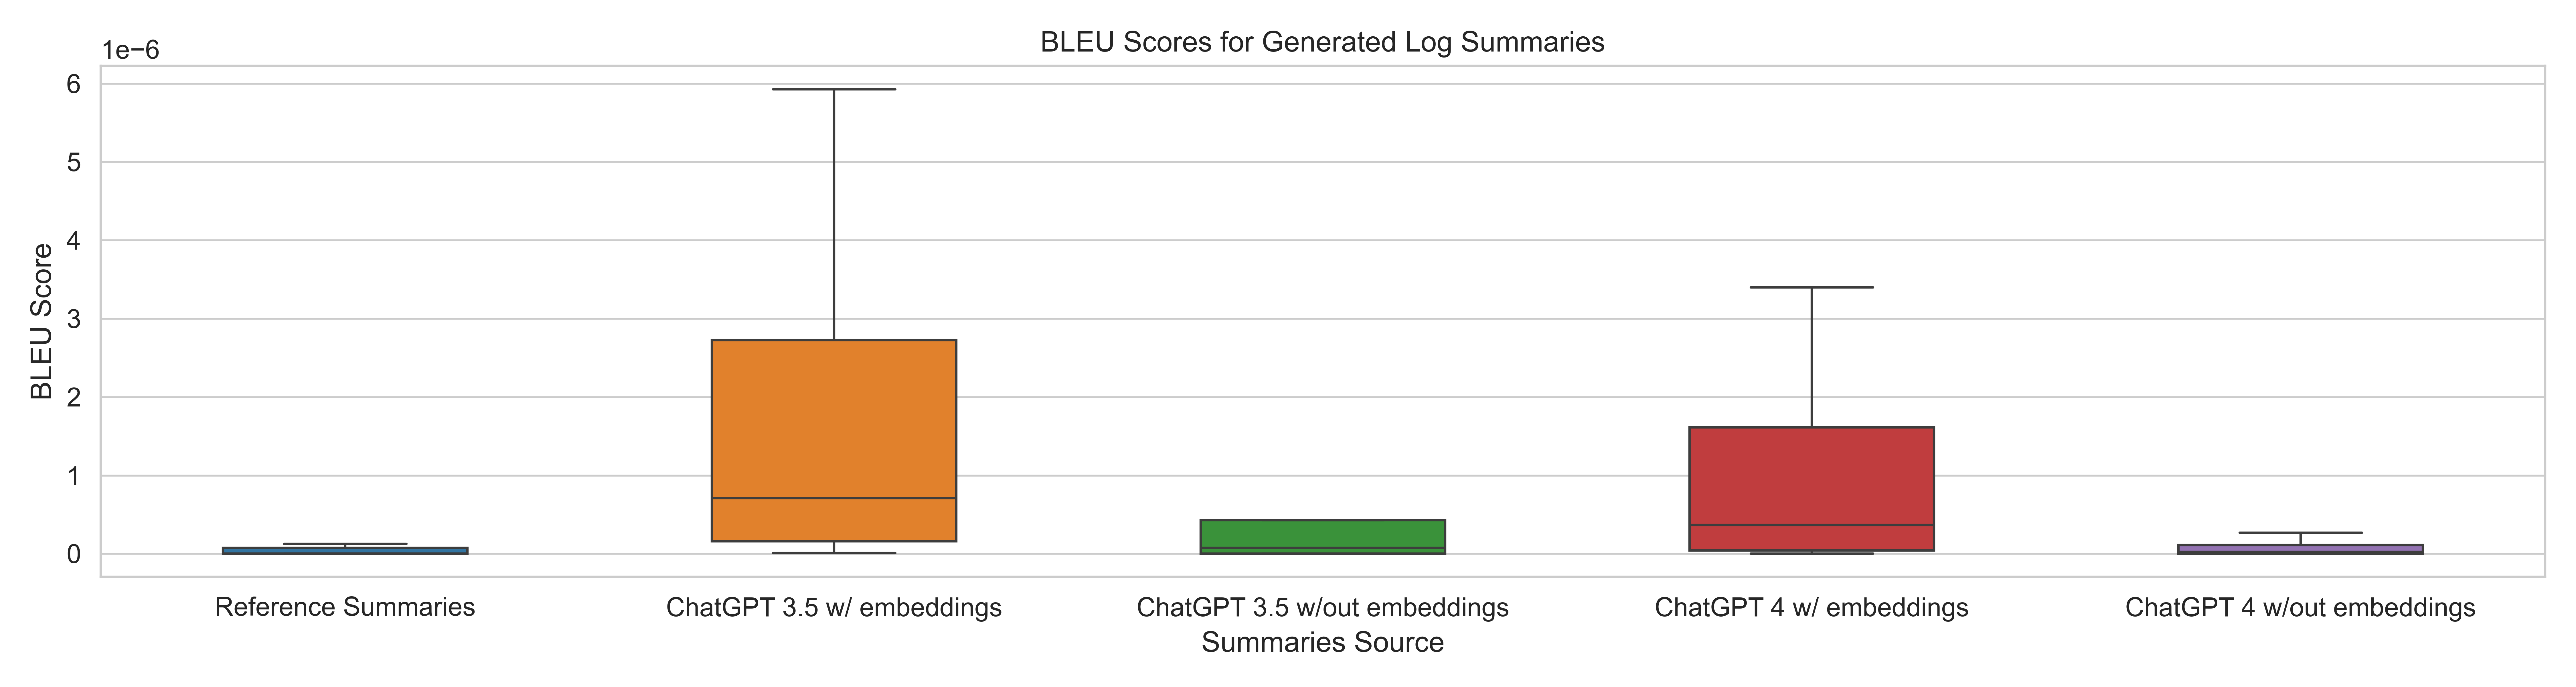
\includegraphics[width=\textwidth]{final/img/results/bleu-scores.png}
    \caption{BLEU Score Results}
    \label{fig:bleu-scores}
\end{subfigure}

\begin{subfigure}{\textwidth}
    \centering
    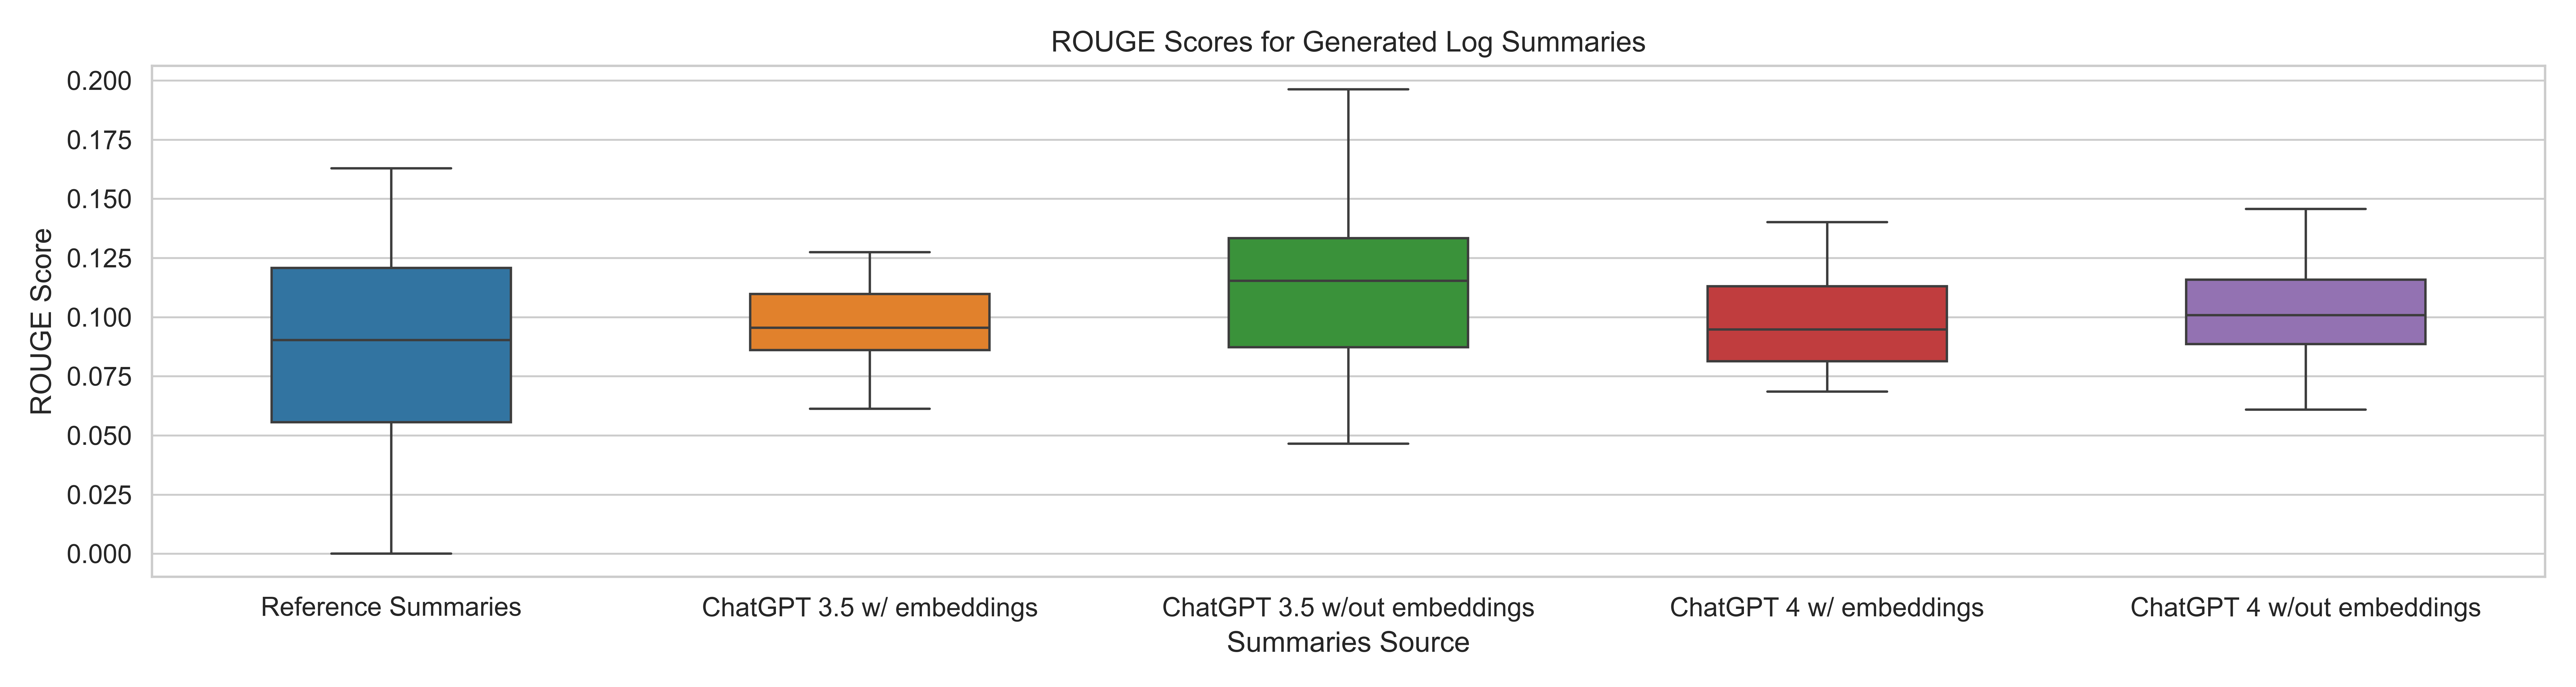
\includegraphics[width=\textwidth]{final/img/results/rouge-scores.png}
    \caption{ROUGE Score Results}
    \label{fig:rouge-scores}
\end{subfigure}

\begin{subfigure}{\textwidth}
    \centering
    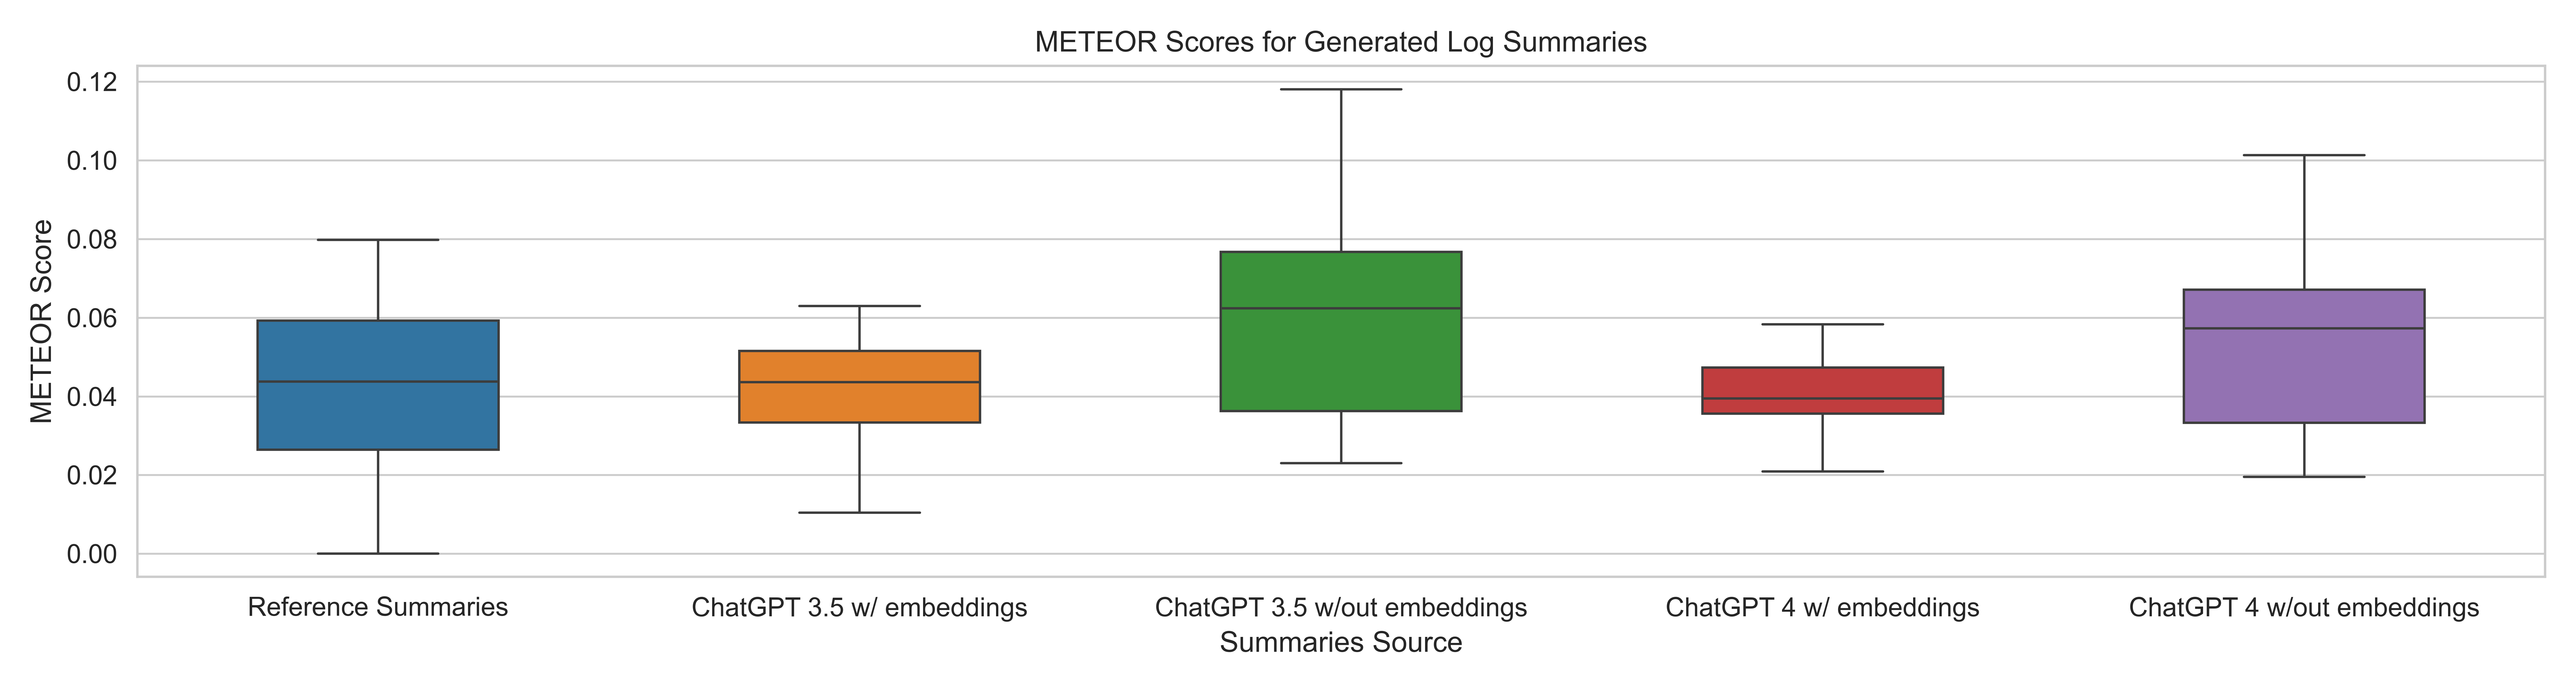
\includegraphics[width=\textwidth]{final/img/results/meteor-scores.png}
    \caption{METEOR Score Results}
    \label{fig:meteor-scores}
\end{subfigure}

\end{figure*}

\begin{figure*}[t]

\begin{subfigure}{\textwidth}
    \centering
    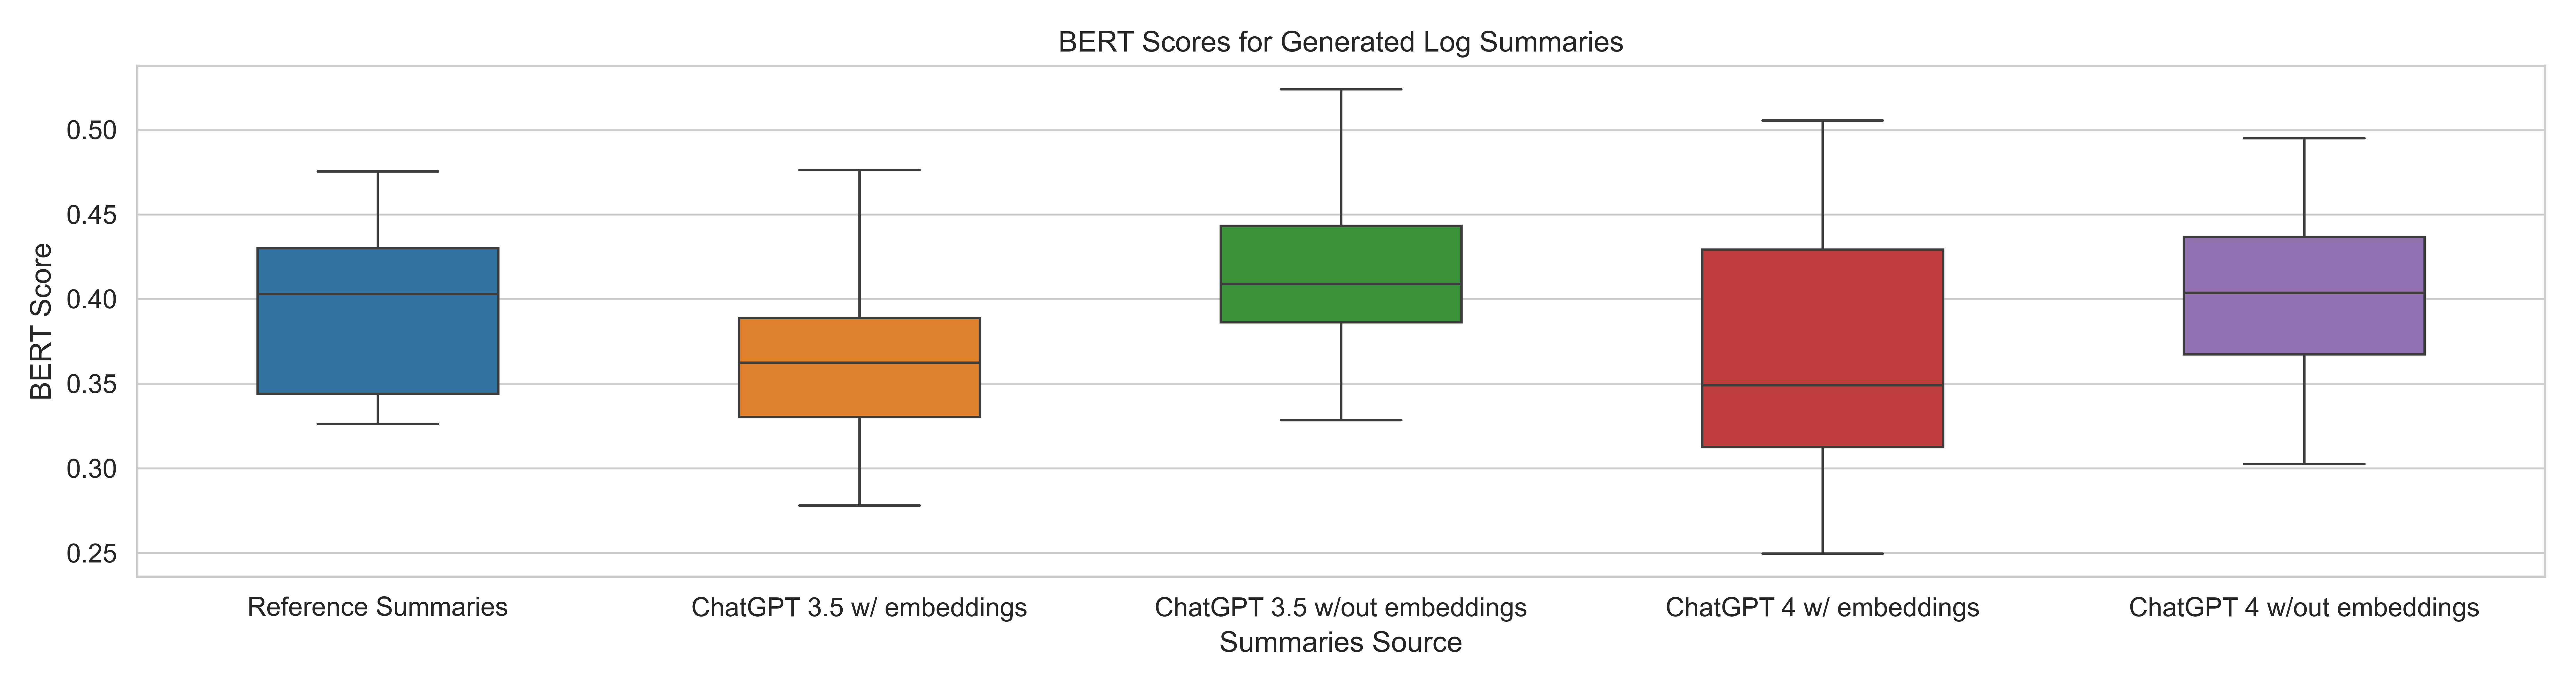
\includegraphics[width=\textwidth]{final/img/results/bert-scores.png}
    \caption{BERT Score Results}
    \label{fig:bert-scores}
\end{subfigure}

\begin{subfigure}{\textwidth}
    \centering
    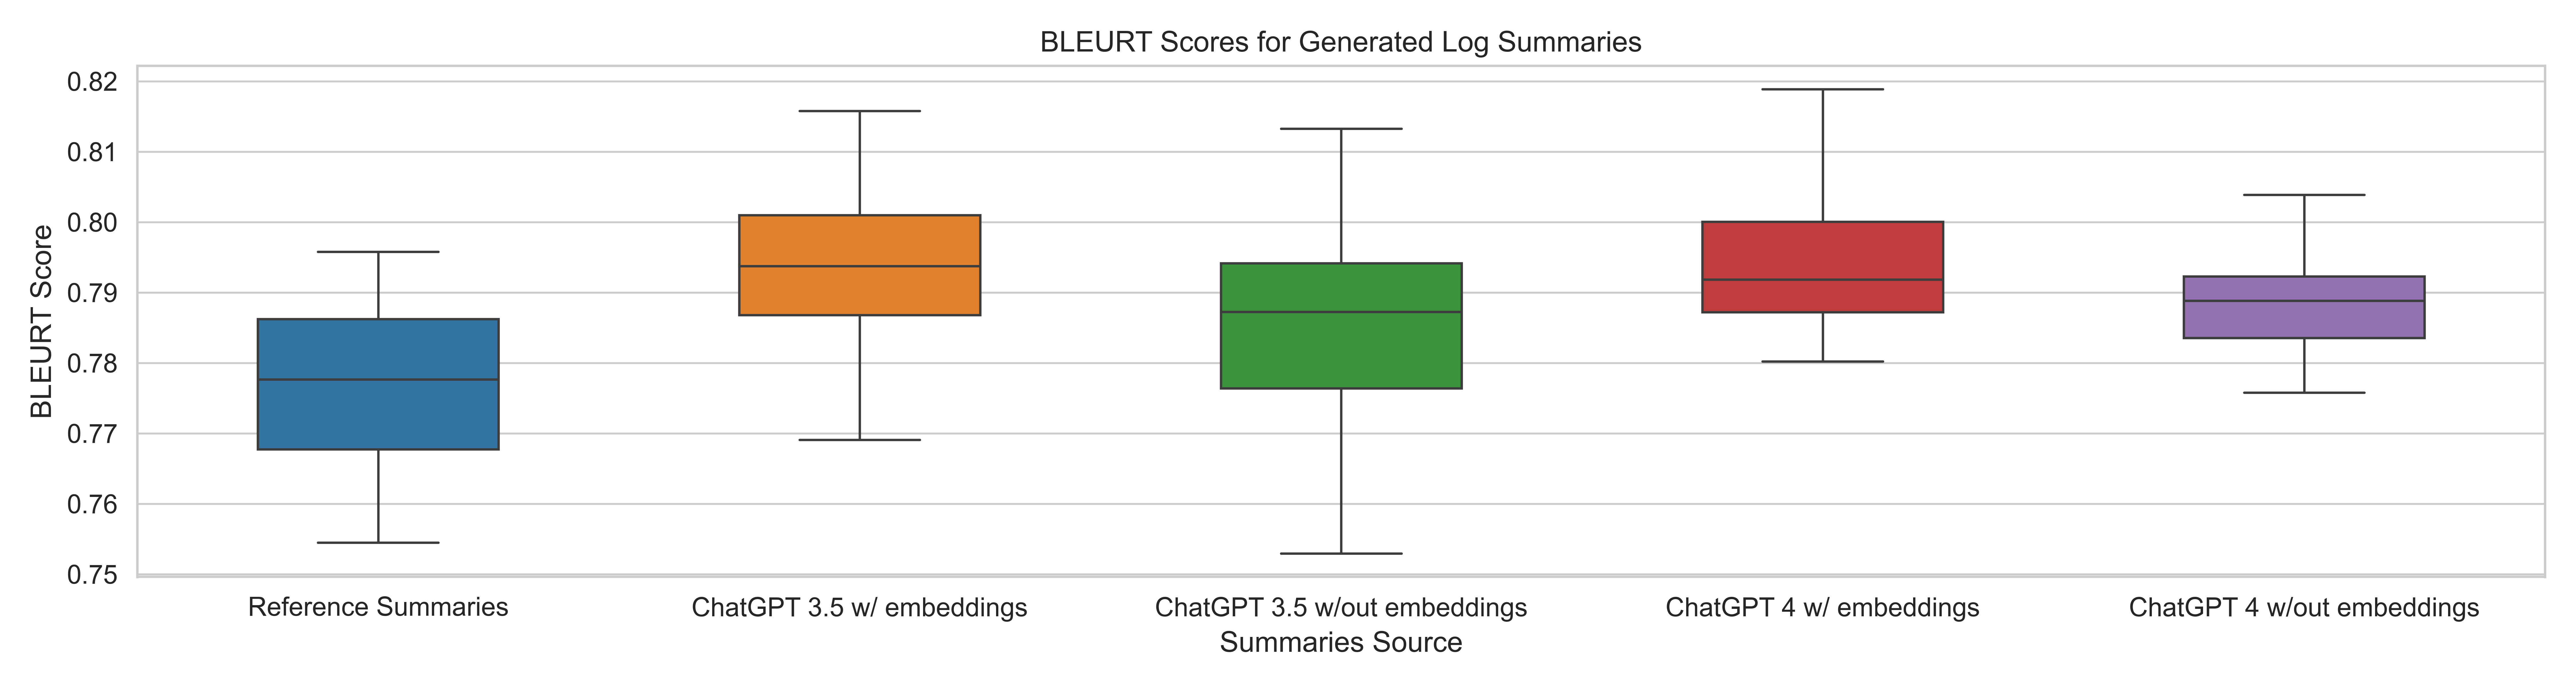
\includegraphics[width=\textwidth]{final/img/results/bleurt-scores.png}
    \caption{BLEURT Score Results}
    \label{fig:bleurt-scores}
\end{subfigure}

\begin{subfigure}{\textwidth}
    \centering
    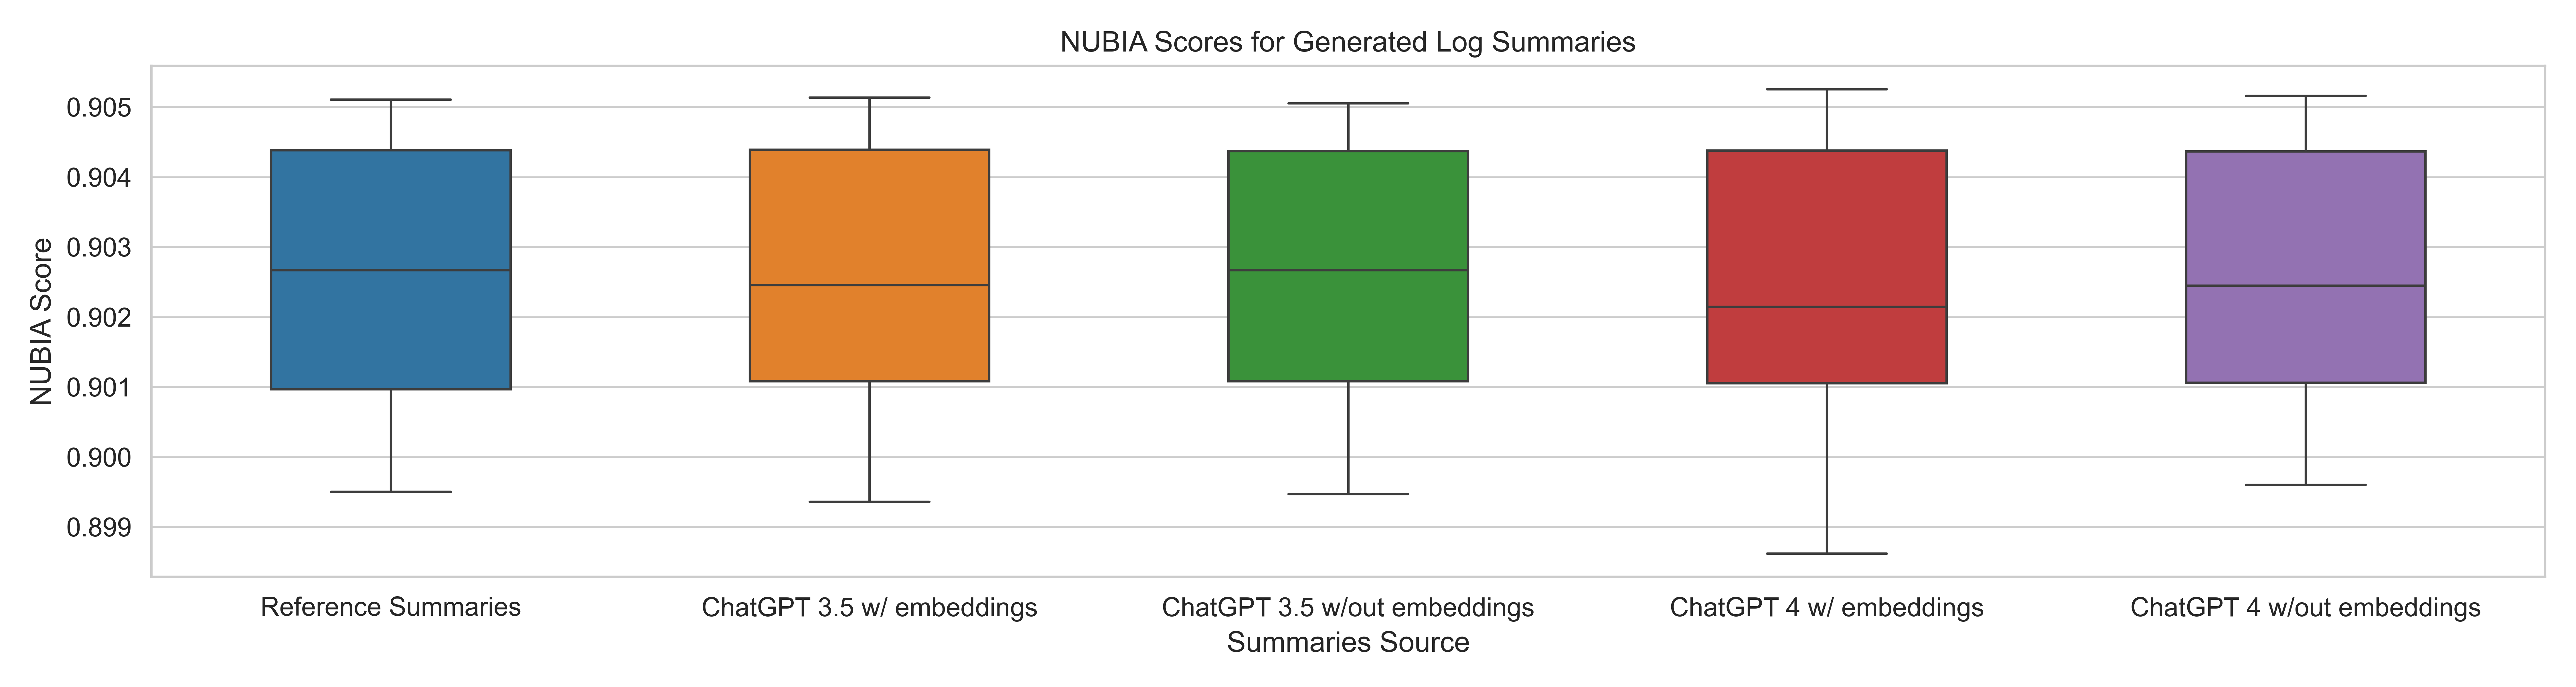
\includegraphics[width=\textwidth]{final/img/results/nubia-scores.png}
    \caption{NUBIA Score Results}
    \label{fig:nubia-scores}
\end{subfigure}
    
\end{figure*}

For the BLUE Score metrics as shown in Figure \ref{fig:bleu-scores},  we observe a wider range when it comes to incorporation with embeddings. However, note that the y-axis in the graph states that it is \(1* e^-6\), so the difference is insignificant.

For the ROUGE Score Results as shown in Figure \ref{fig:rouge-scores}, higher scores indicate higher similarity between the produced summary and reference. We see that there is little difference between the models with and without embeddings. The difference is considered statistically insignificant here.

The METEOR score measures the quality of the generated texts against reference text through the generalized concept of unigram precision and recall. Based on Figure \ref{fig:meteor-scores} we also don't see any noticeable differences between the models with or without embeddings. 

BERT scores, which use the contextual embeddings from BERT and performs a cosine similarity on the matched and reference summary, also does not show a noticeable difference here. From Figure \ref{fig:bert-scores}, we see that the BERT scores are actually slightly worse on ChatGPT4 with embeddings, but the difference is also extremely small. 

The BLEURT Score is a mixture of BLUE and BERT Metrics. It is a novel automatic metric which is much closer to human annotation as it captures non-trivial semantic similarities between two sentences. From the Figure \ref{fig:bleurt-scores}, we observe that the there are some differences between the summaries generated with embeddings and those generated without the embeddings. The summaries generated with embeddings show slightly better BLUERT scores compared to the range of the scores of the summaries generated without embeddings. 

Finally, the last scoring which we use in evaluation is the NUBIA Score. NUBIA Score is a state-of-the-art (SoTA) evaluation metric which is used to measure the quality of generated sentences. It uses three modules: feature extraction, aggregator, and calibration. It uses RoBERTa for capturing semantic similarity and logical inferencing then GPT-2 for sentence legibility. The scoring results from our experiment is shown in Figure \ref{fig:nubia-scores}, where we observe that all generated summaries are in the high range of 0.90+, regardless of which model being used or whether embeddings are included or not.

Overall, all the results show that we do not observe any significant differences between gpt3.5 and gpt4. In the BLUEURT Scores, there is a small difference, suggesting that using embeddings in the prompt offers slightly better performance. This is promising, as the BLEURT score is an improved version of BERT score and addresses the fact that the other popular metrics such as BLEU and ROGUE may produce scores that correlate poorly with human judgement.

\section{Conclusion}

As we have produced some promising results from BLEURT Scores and NUBIA Scores, we believe our system can potentially benefit companies of all sizes and improve their IT Operations workflows in a modern complex cloud infrastructure, as they often are unable to allocate the necessary resources and budget to train and fine-tune large ML models. We expect the following stakeholders to benefit from this project:
\begin{itemize}
    \item Site Reliability Engineers
    \item Platform Engineers 
    \item Management Audience 
    \item Incident Commanders 
\end{itemize}

We expect that SREs and Platform Engineers are the stakeholders that will benefit the most as our framework can used as an assistance tool for SREs when when maintaining cloud systems or responding to cloud incidents. Managers can use this tool to understand the current situation of the infrastructure without knowing many technical details. The incident commander can use this tool to ensure that the analysis is flowing in the right direction. 

We believe it is a great time to incorporate Generative AI into the corporate world within the IT Operations field. We hope this framework can transform how incident management, alerting, and root cause analysis are performed. 

The use of embeddings only slightly improved the BLEURT scores. Given a vector store with more logs and summaries, we expect that the BLEURT scores would be higher when using similar logs/summaries in the prompt. Normally, in the corporate world, there would be much more data available through past incident summaries, and we believe the overall results should be better with incorporating the use of embeddings.

\section{Future Work}

Presently, we do not have a log pre-processing pipeline set up to tokenize logs with a domain-specific tokenizer. Future work would implement such a preprocessing setup so that we can gather the logs with some form of automation and verification.

The lexical scores also does not provide much insights as it does not consider the context of the produced summaries, which often leads to low scores and are not a good measurements. In the future, we plan to incorporate semantic scores only and getting rid of the lexical scores. In addition, we plan to identify other semantic scores that are suitable for the quality assessments. 

For the embeddings, since we are only feeding very limited set of logs and its associated summaries, the similarity scores which we get are sometimes not close to 0, which can mean that it can potentially mislead the ChatGPT to produce inferior results. Future work will incorporate better prompt engineering and the scores of similarity search, to ensure that we only include the results with similarity scores that are closer to 0.

In our example dataset, we only include a snippet of logs and its corresponding summaries, and performed evaluation based on the dataset only. However, in a real-world scenario, this is often not the case as the logs will be mixed with multiple scenarios which would span into multiple summaries. Therefore, we plan to extend our research to a hierarchical summaries of summaries, basically generating a summary out of multiple summaries which would be more closely aligned with what we observe in the typical cloud environment. 


\section{Top 5 conferences or workshops that fits}
The first choice of the conferences which best suits the paper is IEEE Cloud. The IEEE Cloud 2024 is going to be held in Washington DC, and the Paper Submission Deadline is Mar. 1st, 2024, which allows us to refine our experiments further and potentially incorporate some of our future work. In fact, the paper "Learning representations on logs for AIOps" \cite{gupta2023learning} was accepted for IEEE Cloud 2023, and since our research is related to AIOps, we believe that it will result in a higher chance of getting accepted in that conference.

The second choice would be IEEE/ACIS on Big Data, Cloud Computing, and Data Science (BCD 2024). This conference includes topics on Cloud Applications Performance and Monitoring, which the log summary can definitely be used for Cloud applications monitoring. There are both workshops and Paper Submissions that we can consider. The workshops proposal are due this week on Dec. 15, which can be a little tight in terms of the deadline. However, the paper submission is due on Apr. 1, 2024, which will provide us plenty of time to refine our paper for submission.

The third choice would be IEEE International Conference on Cloud Engineering (IC2E), which will be hosted Cyprus in September 2024. The Paper submission deadline is on April 2024, which also provides us plenty of time to refine our paper for submission. The reason why we picked this conference is that our AIOps Research is closely related to cloud applications monitoring, which aligns with the cloud application track for this conference. In particular, our page numbers and formatting fulfills the instructions of the submission instructions from the IC2E 2024 website.

The fourth choice would be CCGRID 2024. This was the suggested conference from our professor and will be hosted on Philadelphia on May 2024. It is likely to meet the criteria of Track 3 of using AI to enhance the reliability of the cluster and cloud computing systems. However, the deadline is actually due for tomorrow, December 11. Which we would probably not make it unless they extend the deadline by another week.

The last choice would be ACM International Conference on Information and Knowledge Management, known as CIKM 2024. This conference is scheduled for Oct 2024 in Boise, Idaho, and can be a little too late for our timing as they have not even determined the submission dates yet. However, as our research closely aligns with their objective of "recent advances on data and knowledge bases", we believe that we have a chance to have our papers getting accepted at this conference.



\clearpage
\bibliographystyle{plain}
\bibliography{ref}
\vspace{12pt}

\end{document}